%%%%%%%%%% TO DO %%%%%%%%%%
% - Add figures for glitches
% - Add figures for omega scans and tools

%%%%%%%%%% %%%%%%%%%% %%%%%%%%%%



% Purpose of the chapter
In this thesis we have made improvements to the search for gravitational waves using a detector characterisation context by improving the quality of the detector data and understanding the noise background of the detectors. 

% Section by section of chapter
In this chapter we will discuss the gravitational wave detectors and the limiting sources of noise in section~\ref{}. We define the research area of detector characterisation in section~\ref{}. We further explain some common characterisation techniques in section~\ref{}, the common noise transients in section~\ref{}, some of the challenges faced in detector characterisation in section~\ref{} and finally the detector characterisation tools most commonly used and referred to throughout this thesis, in section~\ref{}.

\section{\label{3:sec:gw_detectors}Gravitational Wave Detectors}

% To understand the importance of Detector Characterisation we must understand the detectors
Gravitational wave astronomy in the present day is performed by ground-based detectors at different locations globally: the LIGO-Livingston and LIGO-Hanford detectors are located in the United States of America, the Virgo interferometer in Italy and, the KAGRA telescope in Japan. We will primarily reference the LIGO detectors in the United States of America when discussing the challenges faced in detector characterisation. 

As previously mentioned in chapter~\ref{}, section~\ref{}, the LIGO detectors work on the principle of laser interferometry to detect gravitational wave signals. The sensitivity~\cite{aLIGO_design_curve:2018} of Gravitational Wave detectors is limited by fundamental sources of noise such as seismic noise~\cite{Glanzer:2023}, thermal noise~\cite{thermal_noise:2018} and quantum noise~\cite{quantum_noise:2003}. These are the non-stationary sources of noise~\cite{PSD_var:2020}. Additionally, we have non-Gaussian noise~\cite{Noise_Guide:2020} which manifests as transient noise bursts in the data which can contribute to false positives in gravitational wave searches and the obscuring of real gravitational wave signals~\cite{GW170817:2017, GW150914_noise:2016}.

\section{\label{3:sec:detchar_calib}Detector Characterisation and Calibration}

Detector characterisation is a field of study which assess and improves the performance of gravitational wave detectors to ensure accurate and reliable detection of gravitational waves. Gravitational wave detector calibration determines how the response of the detector translates to astrophysical signals, ensuring accuracy in extracted astrophysical information. Detector characterisation is responsible for identifying and mitigating the many sources of noise that can obscure or mimic real signals. The optimisation of detector sensitivity is also studied whereby different designs and components can be fine-tuned to increase sensitivity. Another responsibility of detector characterisation is the monitoring of detector performance in real-time to assess sensitivity changes.

Overall, effective detector characterisation ensures that gravitational wave observatories can achieve their scientific goals by providing accurate and reliable observations of gravitational waves. The gravitational wave detectors have dedicated working groups for detector characterisation and calibration~\cite{O2O3_DetChar:2021, VirgoDetChar:2023}. Chapter~\ref{} is a direct contribution to the field of detector characterisation.

The detector characterisation group has the important task of verifying data quality when a gravitational wave signal is detected in live time, giving the confirmation that the gravitational wave signal isn't a false alarm potentially caused by noise transients or poor data quality immediately surrounding the gravitational wave signal.

\subsection{\label{3:sec:detector-analysis}Detector Analysis}

% Noise analysis
%    Different sources of noise
%    Seismic, thermal, shot, radiation pressure
%    Noise Curve

Systematic sources of noise are the dominating limit in the sensitivity of ground-based detectors. The sources of noise with the greatest contributions are
%
\begin{itemize}
    \item Seismic noise~\cite{Glanzer:2023}: the vibrations of the ground causes a coupled vibration motion in the mirrors of the interferometer. Higher frequency seismic noise ($1-10$Hz) is often caused by local ground movements typically anthropomorphic in nature or greater magnitude earthquakes~\cite{Nuttall:2018}. Lower frequency seismic noise ($<1$Hz) is caused by larger-scale geophysical processes such as: ocean waves, tidal effects, or smaller local earthquakes~\cite{aLIGO:2015}. Seismic noise can be mitigated with advanced suspension systems to isolate mirrors and end-station components from the ground to prevent coupling to seismic motion~\cite{seismic_isolation:2015}.
    \item Thermal noise~\cite{thermal_noise:2018}: the thermal energy of interferometer components will cause them to vibrate. This noise can be reduced with new mirror materials with resonant frequencies outside the sensitive regions or with cryogenically cooled mirrors such as those used by KAGRA~\cite{KAGRA:2021}.
    \item Shot noise~\cite{quantum_noise:2003}: the distribution in the number of photons observed by the interferometer photodetector in any time interval is Poisson distributed and the error in the photon count places limits on the sensitivity. The error is proportional to the square-root of the count ($\sigma = \sqrt{\lambda}$, where $\lambda$ is the photon count and $\sigma$ is the standard-deviation or error) therefore, the simplest way to reduce this error is to increase the laser power and increase the photon count in the time interval.
    \item Radiation pressure~\cite{quantum_noise:2003}: the pressure exerted by the photons hitting the end mirrors will decrease search sensitivity. To reduce this noise the laser power can be reduced however, this will increase the shot noise.
\end{itemize}

It can be seen that the laser power must be calibrated to balance the impact of increasing the photon count which will decrease shot noise but simultaneously increase radiation pressure noise. A figure displaying these systematic noise sources and their limitations in the LIGO detector case can be seen in figure~\ref{3:fig:aLIGO_noise}.
%
\begin{figure}
    \centering
    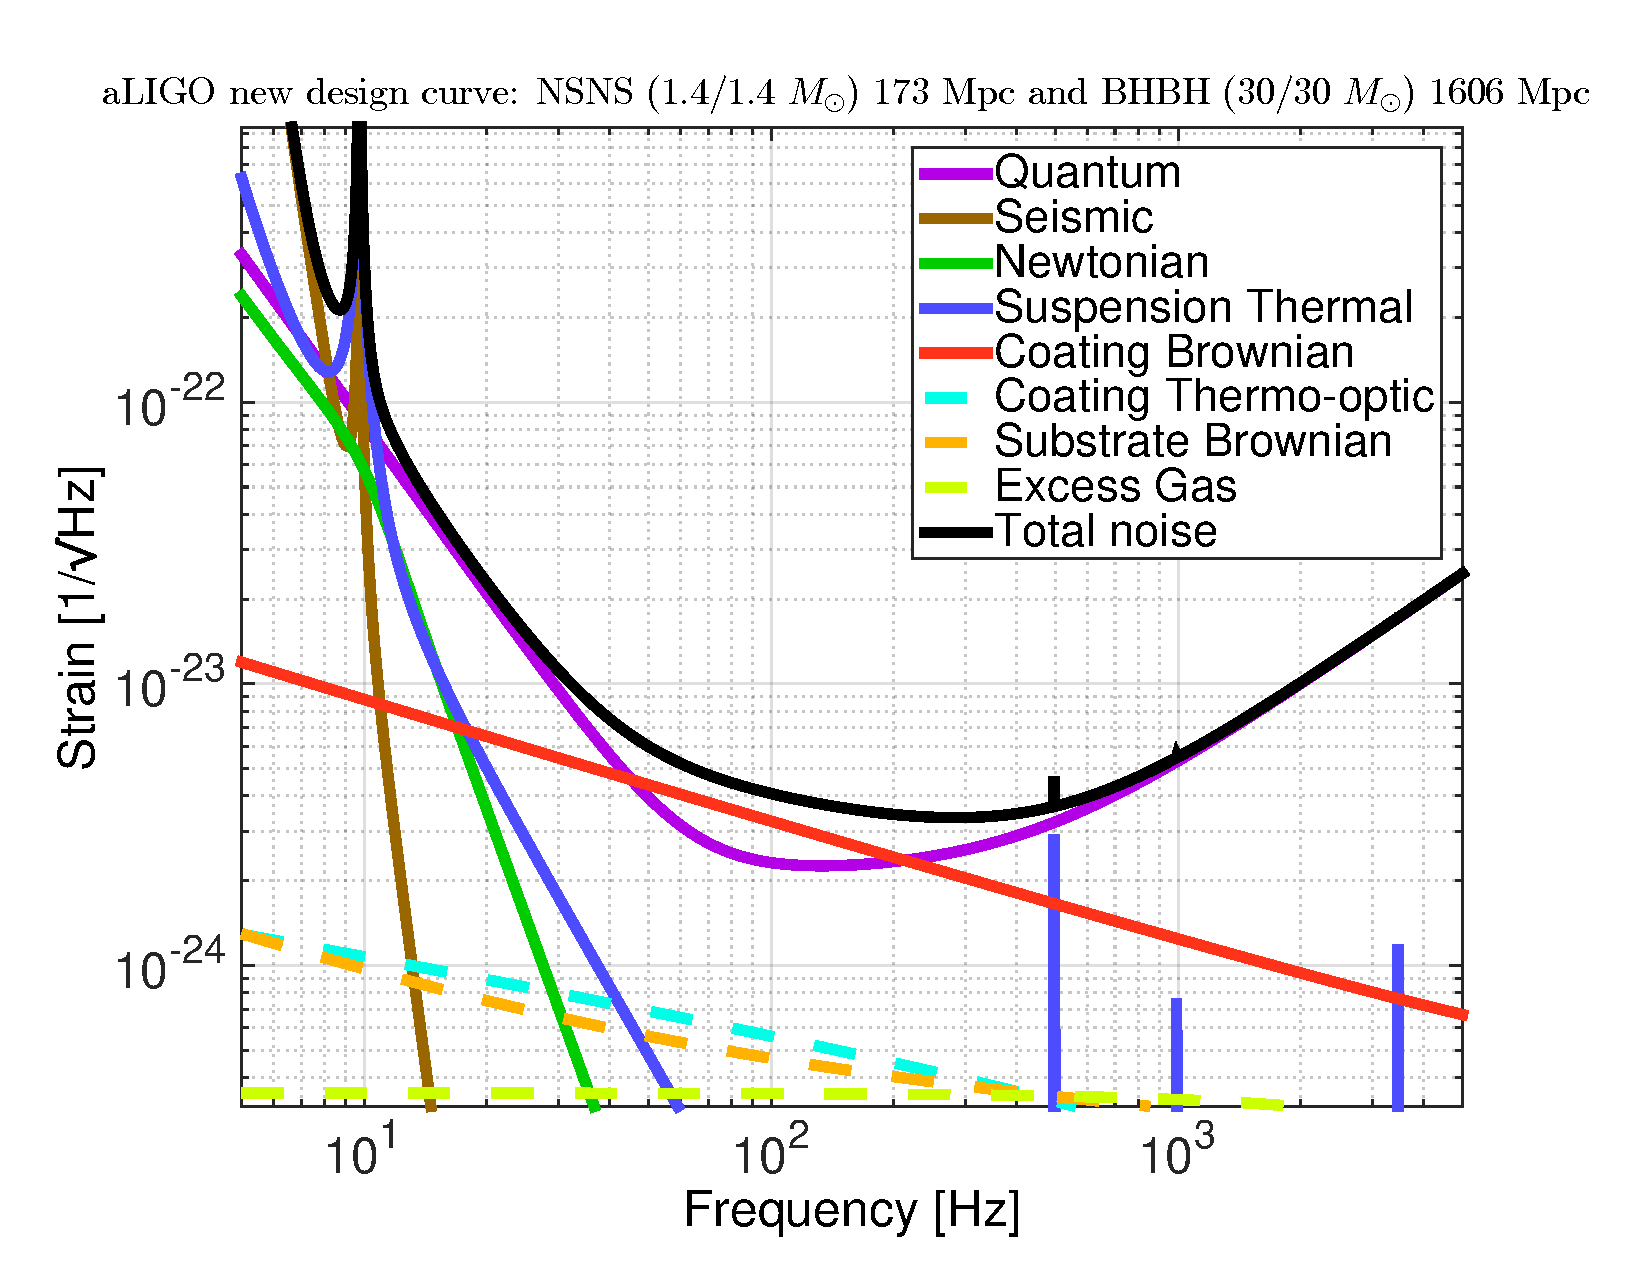
\includegraphics[width=1.0\linewidth]{images/3_detector_characterisation/aLIGO_newDesign.pdf}
    \caption{The Advanced LIGO~\cite{aLIGO:2015} strain sensitivity as a function of frequency (black solid line), accompanied by the systematic noise sources which limit the sensitivity of the detector. Figure originally released in~\cite{aLIGO_design_curve:2018}.}
    \label{3:fig:aLIGO_noise}
\end{figure}
%

% Sensitivity Analysis
%    BNS Distance
%    Sensitivity Measurement
To monitor detector sensitivity the binary neutron star inspiral range is calculated. This is the range at which (in Mpc) a binary neutron star signal with components masses of $1.4$ M$_{\odot}$ will be detected given the characteristic noise (PSD) of the data calculated by taking an average of the detector noise in the previous minute~\cite{range_calculation:2003, ota:2023}. Figure~\ref{3:fig:bns_range} shows an example of the binary neutron star range for a day of LIGO-Hanford during the fourth observing run.
%
\begin{figure}
    \centering
    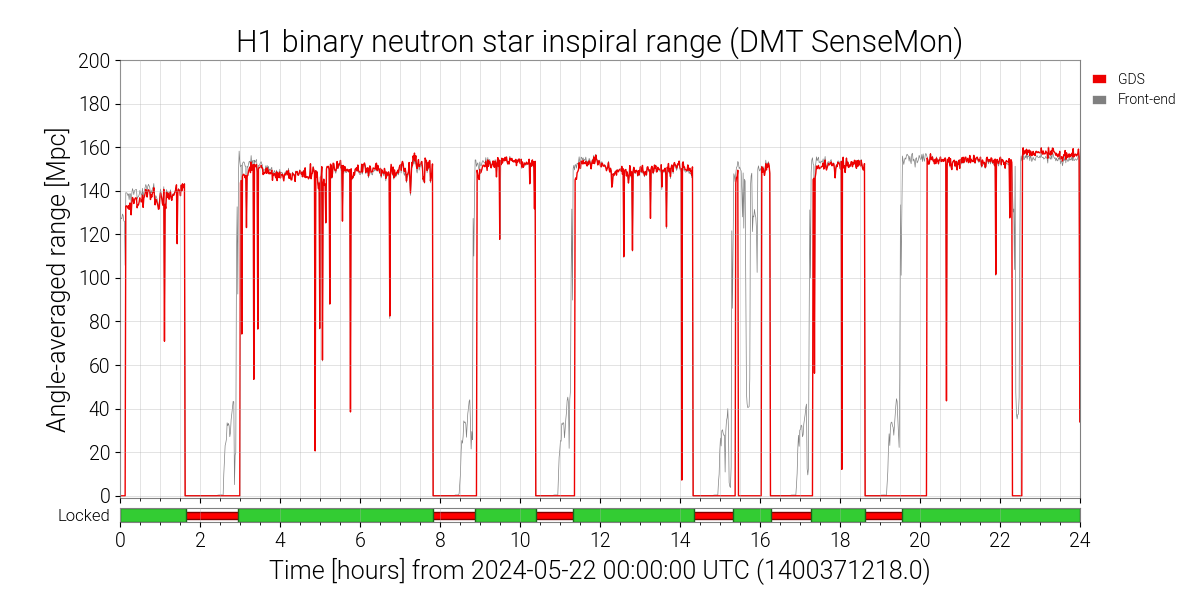
\includegraphics[width=1.0\linewidth]{images/3_detector_characterisation/may22_bns_range.png}
    \caption{The LIGO-Hanford binary neutron star inspiral range for the 22nd May 2024, created using GWSumm~\cite{gwsumm:2024} and taken from the LIGO Summary Pages-\href{https://summary.ligo.org/}{https://summary.ligo.org/}, please see \href{https://gwosc.org/detector_status/}{https://gwosc.org/detector\_status/} for the public summary pages.}
    \label{3:fig:bns_range}
\end{figure}
%

\subsection{\label{3:sec:noise-transients}Noise Transients}

% Introduction to Noise Transients

Noise transients, commonly referred to as glitches, are short duration bursts of noise found in gravitational wave data. The systematic sources of noise described in section~\ref{3:sec:detector-analysis} limit the sensitivity of the detector to a certain frequency range, glitches appear within this sensitivity frequency range. The specific noise transients investigated by detector characterisation are non-Gaussian noise artefacts that have the ability to obscure~\cite{GW170817:2017} or mimic gravitational wave signals~\cite{GWMimicking:2010} producing false-alarms in our gravitational wave search pipelines. Understanding these glitches is crucial for gravitational wave detection, they have the potential to reduce the sensitivity and hinder the reliability of the detectors.
%
% GW170817 Obscured
%

% Characteristics of Noise Transients

There are as many as $24$~\cite{gravityspy:2023} different classes of glitch which all manifest with different durations (typically in the millisecond to second range) and amplitudes. Glitches populate the whole sensitive frequency bandwidth of the detectors with some glitches being broadband, affecting up to the whole frequency bandwidth, to others being narrowband and affecting only specific frequency ranges. Glitches are commonly characterised and studied in 2-dimensional time-frequency representations of the one-dimensional strain time series that the detector outputs. The typical time-frequency representation used is the OmegaScan~\cite{qscan:2004} (also referred to as a Q-scan) which is described later in this chapter.

% Common Sources of Noise Transients

Glitches originate from either environmental sources, instrumental sources or a coupling of the two. As mentioned previously, seismic noise limits the sensitivity of the detectors below $\sim10$Hz, but the coupling of seismic motion into interferometer components can cause one of the more common glitches---scattered light. Other environmental noise sources are heavy winds, lightning, and human activity (traffic, construction, trains, the daily commute). A historical glitch identified at LIGO-Livingston was caused by an air conditioning compressor cycling, these glitches were seen by both a magnetometer and the gravitational wave channel. Other instrumental glitches might be caused by mirror suspensions, electronics, control systems or laser fluctuations.
%
% Figure for scattered light and magnetic noise
%

% Other examples of some common glitches

The most common glitches are: blips~\cite{blips:2019}, scattered light~\cite{ArchEnemy:2023} and whistles~\cite{glitschen:2021}, Omegascans of these glitches can be seen in figure~ADD. The sources of these glitches have been studied, for example, whistles are caused by the beating of radio frequencies in the detector, however, some glitches are from unknown sources such as blips. Scattered light has been found from many different sources in the detector and great effort has been made to reduce the presence of scattered light in the data~\cite{reducing_scattering:2020} but as of the fourth observing run some scattered light still remains.
%
% figure for glitches
%

% Detection and Characterisation of Noise Transients

An number of algorithms and tools have been developed to detect and characterise noise transients in gravitational wave data~\cite{ArchEnemy:2023, reducing_scattering:2020, Glanzer:2023, gravityspy:2017, gravityspy:2021, gravityspy:2023, glitschen:2021,  BayesWave:2015, gwadaptive:2022, O3_subtraction:2022, Powell:2016, glitschen:2021}. The primary aim of these tools is the identification of glitches and analysis of properties of the glitches (amplitude, frequency, duration, waveform shape) to determine the source of the noise. Once the noise source has been identified improvements to the detector can be made to eliminate it. Other tools focus on modelling noise transients for the purpose of subtracting them from affected gravitational wave data~\cite{ArchEnemy:2023, BayesWave:2015, glitschen:2021, antiglitch:2023}.
%
% GravitySpy figure of a bunch of glitch classes
%

% Auxiliary Channels

Another tool to use in the identification and classification of glitches in the thousands of auxiliary channels alongside the main strain channel~\cite{iDQ:2020} which monitor the many subsystems of the detector and can be used to find noise correlations between the different parts of the instrument~\cite{DQ_vetoes:2017}. The auxiliary channels which are not sensitive to gravitational waves are very useful in identifying any correlations between noise in the gravitational strain channel and noise also seen in another channel which cannot observe gravitational waves, an example of this is the magnetometer recording the same glitch as seen in the grvaitational wave strain channel when the air conditioning compressor was cycling at LIGO-Livingston~\cite{Nuttall:2018}.

\subsection{\label{3:sec:detchar-tools}Detector Characterisation Tools}
%%%%% to do %%%%%%%%
\paragraph{Omega-scan}

is a whitened spectrogram with a high time and frequency resolution, created by the \verb|gwdetchar-omega|. These are the most common way to visualise the time series data in the time-frequency plane which can reveal key time-frequency relationships that are virtually impossible for a human to see in the time series. For a given event time \verb|gwdetchat-omega| is used by the detector characterisation group to visually identify any glitches in the data. An example of an omega-scan can be seen in figure~ADD.
%
%figure of an omega-scan

\paragraph{GravitySpy}

is a citizen science machine learning tool for classifying glitches found in gravitational wave data~\cite{gravityspy:2017}. GravitySpy has been trained by volunteers on the website~ADD and the project itself can be found at~ADD.

GravitySpy takes millions of omega-scans of gravitational wave data which have been found to contain bursts of power. These omega-scans are images which potentially contain glitches, they are published on the GravitySpy project and volunteers are given these images and the option for which glitch they think is contained within the image. Once millions of these images have been classified the machine learning algorithm is trained and it can go further to classify the images without the need of volunteers~\cite{gravityspy:2021}.

GravitySpy was run on data from the second and third observing runs, where it was able to classify 23 different glitch categories. The downsides of GravitySpy are the constantly changing noise background of the gravitational wave detectors and the new glitch types emerging which need to be trained on with volunteering again~\cite{gravityspy:2023}.

Further extensions have been made to GravitySpy with new machine learning architecture which are capable of retraining on new glitch types without needing the volunteering. They are also able to do this and that and everything else: GWSpyTreeThing~\cite{GSpyNetTree:2023}


\paragraph{Data Quality Vetoes}

are used by the gravitational wave searches and are a flags applied to periods of data which contain potential data quality issues~\cite{DQ_vetoes:2017}. These periods of data are identified using tools such as \verb|Omicron| and when applied to the searches there is a significant reduction in the number of high SNR triggers that would've been found during these times.

The data quality vetoes are constructed using auxiliary channel information which has been found to be strongly correlated to instrumental noise. An example is a significantly elevated transient noise rate in the strain channel five days prior to GW150914~\cite{GW150914:2016} which was traced back to the 45MHz electro-optic modulator driver system used to generate optical cavity control feedback signals~\cite{aLIGO:2015}. The noise caused by this channel was given a category 1 veto data quality flag and removed 2.62\% of the total coincident time from the analysis period.

\paragraph{iDQ}

is another tools used to generate data quality flags which are used in the gravitational wave searches~\cite{iDQ:2020}. iDQ is a supervised learning framework which autonomously detects glitches based only on the auxiliary channels which are insensitive to gravitational waves---meaning these channels will only see glitches and not gravitational wave radiation. iDQ operates in low-latency and is used in the live gravitational wave searches to provide data quality information in real-time. This tool is invaluable for low latency searches to prevent significant contamination from high power bursts of noise that would contaminate the searches~\cite{LIGO_data_quality:2015}.

